\chapter{Dasar Teori}
\label{chap:dasarTeori}

Pada bab ini dijelaskan mengenai ....

\section{Morfologi}
\label{sec:morfologi}

Secara etimologi, kata \textit{morfologi} berasal dari kata \textit{morf} yang berarti 'bentuk' dan kata \textit{logi} yang berarti 'ilmu'\cite{chaer:08:morfologi}. Secara harfiah, kata \textit{morfologi} berarti 'ilmu mengenai bentuk'. Di dalam kajian linguistik, \textit{morfologi} berarti 'ilmu mengenai bentuk-bentuk dan pembentukan kata'; sedangkan di dalam kajian biologi, \textit{morfologi} berarti 'ilmu mengenai bentuk-bentuk sel-sel tumbuhan atau jasad-jasad hidup'. Kesamaan dari dua bidang kajian tersebut adalah keduanya mengkaji tentang bentuk. 

Jika morfologi dalam kajian linguistik membicarakan tentang bentuk-bentuk dan pembentukan kata, maka segala bentuk dan jenis morfem yang merupakan satuan bentuk sebelum menjadi kata perlu dibicarakan juga. Pembicaraan mengenai pembentukan kata akan melibatkan pembicaraan mengenai komponen atau unsur pembentukan kata, yaitu morfem, baik morfem dasar maupun morfem afiks, dengan berbagai alat proses pembentukan kata, yaitu afiks dalam proses pembentukan kata melalui proses afiksasi, duplikasi atau pengulangan dalam proses pembentukan kata melalui proses reduplikasi, penggabungan dalam proses pembentukan kata melalui proses komposisi, dan sebagainya. 

Ujung dari proses morfologi adalah terbentuknya \textit{kata} dalam bentuk dan makna sesuai dengan keperluan dalam satu tindak pertuturan. Bila bentuk dan makna yang terbentuk dari satu proses morfologi sesuai dengan yang diperlukan dalam pertuturan, maka bentuknya dapat dikatakan berterima; tetapi jika tidak sesuai dengan yang diperlukan, maka bentuk itu dikatakan tidak berterima. Keberterimaan atau ketidakberterimaan bentuk itu dapat juga karena alasan sosial.


%\subsection{Morfologi dalam Linguistik}
%\label{sec:morfologiLinguistik}

%Di dalam hierarki linguistik, kajian morfologi berada di antara kajian fonologi dan sintaksis seperti tampak pada gambar \ref{gambar-hierarki-linguistik} berikut:

%\begin{figure}[H]
%\centering
%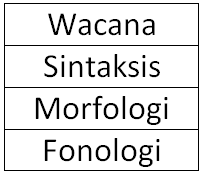
\includegraphics[scale=0.75]{Gambar/gambar-hierarki-linguistik}
%\caption[Hierarki linguistik]{Hierarki linguistik\cite{chaer:08:morfologi}} 
%\label{gambar-hierarki-linguistik}
%\end{figure}

%Sebagai kajian yang terletak di antara kajian fonologi dan sintaksis, maka kajian morfologi mempunyai kaitan baik dengan fonologi maupun dengan sintaksis. Keterkaitan antara morfologi dan fonologi tampak dengan adanya kajian yang disebut dengan \textit{morfonologi} atau \textit{morfofonemik} yaitu ilmu yang mengkaji terjadinya perubahan fonem akibat adanya proses morfologi. Keterkaitan antara morfologi dan sintaksis tampak dengan adanya kajian yang disebut \textit{morfosintaksis} (gabungan dari kata \textit{morfologi} dan \textit{sintaksis}). Keterkaitan ini muncul karena adanya masalah morfologi yang perlu dibicarakan bersama dengan masalah sintaksis. Misalnya, satuan bahasa yang disebut \textit{kata} merupakan satuan terbesar dalam kajian morfologi, sedangkan dalam kajian sintaksis merupakan satuan terkecil dalam pembentukan kalimat atau satuan sintaksis lainnya. Jadi, satuan bahasa yang disebut \textit{kata} itu menjadi objek dalam kajian morfologi dan kajian sintaksis. Dalam gambar \ref{gambar-objek-kajian-linguistik} dapat dilihat kedudukan \textit{kata} dalam keseluruhan objek kajian linguistik.
%
%\begin{figure}[H]
%\centering
%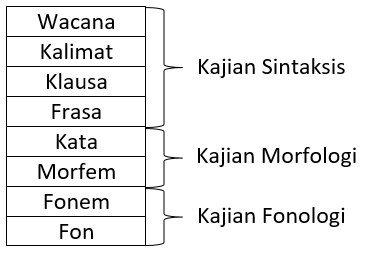
\includegraphics[scale=0.75]{Gambar/gambar-objek-kajian-linguistik}
%\caption[Objek kajian linguistik]{Objek kajian linguistik\cite{chaer:08:morfologi}} 
%\label{gambar-objek-kajian-linguistik}
%\end{figure}
%
%\textbf{Keterangan singkat}
%
%\textit{Wacana} adalah satuan bahasa terbesar atau tertinggi, yang berisi satu satuan ujaran yang lengkap dan utuh; dan dibangun oleh kalimat atau kalimat-kalimat yang dihubungkan secara kohesi dan koherensi.
%
%\textit{Kalimat} adalah satuan sintaksis yang dibangun oleh konstituen dasar (biasanya berupa klausa), dilengkapi dengan konjungsi (bila diperlukan), disertai dengan intonasi final (deklaratif, interogatif, imperatif, atau interjektif).
%
%\textit{Klausa} adalah satuan sintaksis yang berinti adanya sebuah predikat dan adanya fungsi lainnya. Maka sering dikatakan klausa adalah konstruksi yang bersifat predikatif.
%
%\textit{Frase} adalah satuan sintaksis berupa kelompok kata yang posisinya tidak melewati batas fungsi sintaksis (subjek, predikat, objek, atau keterangan).
%
%\textit{Kata} dalam sintaksis merupakan satuan terkecil yang biasa dan dapat menduduki salah satu fungsi sintaksis (subjek, predikat, objek, atau keterangan); dalam morfologi merupakan satuan terbesar, dibentuk melalui salah satu proses morfologi (afiksasi, reduplikasi, komposisi, akronimisasi, dan konversi).
%
%\textit{Morfem} adalah satuan gramatikal terkecil yang bermakna (secara inheren).
%
%\textit{Fonem} adalah satuan bunyi terkecil (dalam kajian fonologi) yang dapat membedakan makna kata.
%
%\textit{Fon} adalah satuan bunyi bahasa yang dilihat tanpa memperhatikan statusnya sebagai pembeda makna kata (dalam kajian fonetik).
%
%
%\subsection{Objek Kajian Morfologi}
%\label{sec:objekKajianMorfologi}

Objek kajian morfologi adalah satuan-satuan morfologi, proses-proses morfologi, dan alat-alat dalam proses morfologi itu\cite{chaer:08:morfologi}. Satuan morfologi adalah:

\begin{enumerate}
	\item Morfem (akar atau afiks).
	\item Kata.
\end{enumerate}

Lalu, proses morfologi melibatkan komponen:

\begin{enumerate}
	\item Dasar (bentuk dasar).
	\item Alat pembentuk (afiks, duplikasi, komposisi).
	%\item Makna gramatikal.
\end{enumerate}

\textit{Morfem} adalah satuan gramatikal terkecil yang bermakna. Morfem dapat berupa akar (dasar) dan dapat pula berupa afiks. Perbedaannya, morfem berupa akar dapat menjadi dasar dalam pembentukan kata, sedangkan morfem berupa afiks hanya "menjadi" penyebab terjadinya makna gramatikal. Kemudian, \textit{kata} adalah satuan gramatikal yang terjadi sebagai hasil dari proses morfologis. Jika berdiri sendiri, setiap kata memiliki makna leksikal dan dalam kedudukannya dalam satuan ujaran memiliki makna gramatikal.

Dalam proses morfologi, dasar atau bentuk dasar merupakan bentuk yang mengalami proses morfologi. Dasar ini dapat berupa sebuah kata dasar maupun bentuk polimorfemis (bentuk berimbuhan, bentuk ulang, atau bentuk gabungan). Alat pembentuk kata dapat berupa afiks dalam proses afiksasi, pengulangan dalam proses reduplikasi, dan penggabungan dalam proses komposisi. 

%Makna gramatikal adalah makna yang "muncul" dalam proses gramatika. Makna gramatikal ini biasa didikotomikan dengan makna leksikal, yakni makna yang secara inheren dimiliki oleh sebuah leksem, yang merupakan satuan dari leksikon. Makna gramatikal ini mempunyai hubungan dengan komponen makna leksikal setiap dasar (akar).


\section{Morfem}
\label{sec:morfem}

Morfem adalah satuan gramatikal terkecil yang memiliki makna\cite{chaer:08:morfologi}. Dengan kata terkecil berarti "satuan" itu tidak dapat dianalisis menjadi lebih kecil lagi tanpa merusak maknanya. Sebagai contoh, bentuk \textit{membeli} dapat dianalisis menjadi dua bentuk terkecil yaitu $\lbrace$me-$\rbrace$ dan $\lbrace$beli$\rbrace$. Bentuk $\lbrace$me-$\rbrace$ adalah sebuah morfem, yakni morfem afiks yang secara gramatikal memiliki sebuah makna; dan bentuk $\lbrace$beli$\rbrace$ juga sebuah morfem, yakni morfem dasar yang secara leksikal memiliki makna. Kalau bentuk \textit{beli} dianalisis menjadi lebih kecil lagi menjadi \textit{be-} dan \textit{li}, keduanya tidak memiliki makna apapun. Jadi, keduanya bukan morfem. Contoh lain, bentuk \textit{berpakaian} dapat dianalisis ke dalam satuan-satuan terkecil menjadi $\lbrace$ber-$\rbrace$, $\lbrace$pakai$\rbrace$, dan $\lbrace$-an$\rbrace$. Ketiganya adalah morfem, di mana $\lbrace$ber-$\rbrace$ adalah morfem prefiks, $\lbrace$pakai$\rbrace$ adalah morfem dasar, dan $\lbrace$-an$\rbrace$ adalah morfem sufiks. Ketiganya memiliki makna. Morfem $\lbrace$ber-$\rbrace$ dan morfem $\lbrace$-an$\rbrace$ memiliki makna gramatikal, sedangkan morfem $\lbrace$pakai$\rbrace$ memiliki makna leksikal. Perlu dicatat dalam konvensi linguistik sebuah bentuk dinyatakan sebagai morfem ditulis dalam kurung kurawal ($\lbrace$...$\rbrace$).


\subsection{Identifikasi Morfem}
\label{sec:identifikasiMorfem}

Satuan bahasa merupakan komposit antara bentuk dan makna\cite{chaer:08:morfologi}. Oleh karena itu, untuk menetapkan sebuah bentuk adalah morfem atau bukan didasarkan pada kriteria bentuk dan makna tersebut. Hal-hal berikut dapat menjadi pedoman untuk menentukan apakah sebuah bentuk adalah morfem atau bukan. 

\begin{enumerate}
	\item Dua bentuk yang sama atau lebih memiliki makna yang sama merupakan sebuah morfem. Umpamanya kata \textit{bulan} pada ketiga kalimat berikut adalah sebuah morfem yang sama.
	\begin{itemize}
		\item \textit{Bulan} depan dia akan menikah.
		\item Sudah tiga \textit{bulan} dia belum bayar uang SPP.
		\item \textit{Bulan} November lamanya 30 hari.
	\end{itemize}
	
	\item Dua bentuk yang sama atau lebih bila memiliki makna yang berbeda merupakan dua morfem yang berbeda. Misalnya kata \textit{bunga} pada kedua kalimat berikut adalah dua buah morfem yang berbeda.
	\begin{itemize}
		\item Bank Indonesia memberi \textit{bunga} 5 persen per tahun.
		\item Dia datang membawa seikat \textit{bunga}.
	\end{itemize}
	
	\item Dua buah bentuk yang berbeda, tetapi memiliki makna yang sama, merupakan dua morfem yang berbeda. Umpamanya, kata \textit{ayah} dan kata \textit{bapak} pada kedua kalimat berikut adalah dua morfem yang berbeda.
	\begin{itemize}
		\item \textit{Ayah} pergi ke Medan.
		\item \textit{Bapak} baru pulang dari Medan.
	\end{itemize}
	
	\item Bentuk-bentuk yang mirip (berbeda sedikit) tetapi maknanya sama adalah sebuah morfem yang sama, asal perbedaan bentuk itu dapat dijelaskan secara fonologis. Umpamanya, bentuk-bentuk \textit{me-}, \textit{mem-}, \textit{men-}, \textit{meny-}, \textit{meng-}, dan \textit{menge-} pada kata-kata berikut adalah sebuah morfem yang sama.
	\begin{itemize}
		\item \textit{me}lihat
		\item \textit{mem}bina
		\item \textit{men}dengar
		\item \textit{meny}usul
		\item \textit{meng}ambil
		\item \textit{menge}cat
	\end{itemize}
	
	\item Bentuk yang hanya muncul dengan pasangan satu-satunya adalah sebuah morfem juga. Umpamanya bentuk \textit{renta} pada konstruksi \textit{tua renta}, dan bentuk \textit{kuyup} pada konstruksi \textit{basah kuyup} adalah juga morfem. Contoh lain, bentuk \textit{bugar} pada \textit{segar bugar}, dan bentuk \textit{mersik} pada \textit{kering mersik}.
	
	\item Bentuk yang muncul berulang-ulang pada satuan yang lebih besar apabila memiliki makna yang sama adalah juga merupakan morfem yang sama. Misalnya bentuk \textit{baca} pada kata-kata berikut adalah sebuah morfem yang sama.
	\begin{itemize}
		\item mem\textit{baca}
		\item pem\textit{baca}
		\item pem\textit{baca}an
		\item \textit{baca}an
		\item ter\textit{baca}
		\item keter\textit{baca}an
	\end{itemize}
	
	\item Bentuk yang muncul berulang-ulang pada satuan bahasa yang lebih besar, apabila mempunyai bentuk bahasa yang sama namun maknanya berbeda (polisemi) merupakan morfem yang sama. Umpamanya, kata \textit{kepala} pada kalimat-kalimat berikut memiliki makna yang berbeda, tetapi tetap merupakan morfem yang sama.
	\begin{itemize}
		\item Ibunya menjadi \textit{kepala} sekolah di sana.
		\item Nomor teleponnya tertera pada \textit{kepala} surat itu.
		\item \textit{Kepala} jarum itu terbuat dari plastik.
		\item Setiap \textit{kepala} mendapat bantuan sepuluh ribu rupiah.
		\item Tubuhnya memang besar tetapi sayang \textit{kepala}nya kosong.
	\end{itemize}
\end{enumerate}


%\subsection{Alomorf dan Morf}
%\label{sec:alomorfDanMorf}
%
%Morfem sebenarnya merupakan barang abstrak karena ada dalam konsep. Sedangkan yang konkret, yang ada dalam pertuturan adalah alomorf, yang tidak lain adalah realisasi dari morfem itu\cite{chaer:08:morfologi}. Jadi, sebagai realisasi dari morfem itu, alomorf ini bersifat nyata/ada. Umpamanya morfem $\lbrace$kuda$\rbrace$ direalisasikan dalam bentuk unsur leksikal \textit{kuda}, dan morfem $\lbrace$-kan$\rbrace$ direalisasikan dalam bentuk sufiks \textit{-kan} seperti terdapat pada \textit{meluruskan} atau \textit{membacakan}.
%
%Pada umumnya sebuah morfem hanya memiliki sebuah alomorf. Namun, ada juga morfem yang direalisasikan dalam beberapa bentuk alomorf. Misalnya, morfem $\lbrace$ber-$\rbrace$ memiliki tiga bentuk alomorf, yaitu \textit{ber-}, \textit{be-}, dan \textit{bel-}, seperti tampak pada tabel \ref{alomorfBer} berikut.
%
%\begin{table}[H]
%\centering
%\begin{tabular}{|c|c|c|}
%\hline
%Morfem & Alomorf & Contoh (pada kata) \\
%\hline
%\textit{ber-} & ber- & bertemu, berdoa \\
%&be-&beternak, bekerja \\
%&bel&belajar. \\
%\hline
%\end{tabular}
%\caption{Bentuk alomorf dari morfem $\lbrace$ber-$\rbrace$\cite{chaer:08:morfologi}}
%\label{alomorfBer}
%\end{table}
%
%Contoh lain, morfem $\lbrace$me-$\rbrace$ memiliki enam buah alomorf seperti tampak pada tabel \ref{alomorfMe} berikut.
%
%\begin{table}[H]
%\centering
%\begin{tabular}{|c|c|c|}
%\hline
%Morfem & Alomorf & Contoh (pada kata) \\
%\hline
%\textit{me-} & me- & melihat, merawat. \\
%&mem-&membaca, membawa, \\
%&men-&menduga, mendengar, \\
%&meny-&menyisir, menyusul, \\
%&meng-&menggali, mengebor, \\
%&menge-&mengecat, mengetik \\
%\hline
%\end{tabular}
%\caption{Bentuk alomorf dari morfem $\lbrace$me-$\rbrace$\cite{chaer:08:morfologi}}
%\label{alomorfMe}
%\end{table}
%
%Di samping istilah \textit{morfem} dan \textit{alomorf} ada pula istilah \textit{morf}. Dalam kajian morfologi, morf berarti bentuk yang belum diketahui statusnya, apakah sebagai morfem atau sebagai alomorf. Jadi, sebenarnya wujud fisik morf adalah sama dengan wujud fisik alomorf. Sedangkan morfem merupakan "abstraksi" dari alomorf atau alomorf-alomorf yang ada. 


\subsection{Jenis Morfem}
\label{sec:jenisMorfem}

Dalam kajian morfologi biasanya dibedakan adanya beberapa morfem berdasarkan kriteria tertentu, seperti kriteria kebebasan, keutuhan, makna, dan sebagainya. Berikut adalah jenis-jenis morfem tersebut.

\begin{enumerate}
	\item Berdasarkan kebebasannya untuk dapat digunakan langsung dalam pertuturan, dibedakan adanya \textit{morfem bebas} dan \textit{morfem terikat}. Morfem bebas adalah morfem yang tanpa keterkaitannya dengan morfem lain dapat langsung digunakan dalam pertuturan. Misalnya, morfem $\lbrace$pulang$\rbrace$, $\lbrace$merah$\rbrace$, dan $\lbrace$pergi$\rbrace$. Morfem bebas ini tentunya berupa morfem dasar. Sedangkan morfem terikat adalah morfem yang harus terlebih dahulu bergabung dengan morfem lain untuk dapat digunakan dalam pertuturan. Dalam hal ini, semua afiks dalam bahasa Indonesia termasuk morfem terikat. Di samping itu, banyak juga morfem terikat yang berupa morfem dasar, seperti $\lbrace$henti$\rbrace$, $\lbrace$juang$\rbrace$, dan $\lbrace$geletak$\rbrace$. Untuk dapat digunakan, ketiga morfem ini harus terlebih dahulu diberi afiks atau digabung dengan morfem lain. Misalnya $\lbrace$juang$\rbrace$ menjadi \textit{berjuang}, \textit{pejuang}, dan \textit{daya juang}; \textit{henti} harus digabung dulu dengan afiks tertentu seperti menjadi \textit{berhenti}, \textit{perhentian}, dan \textit{menghentikan}; dan \textit{geletak} harus diberi imbuhan dulu, misalnya menjadi \textit{tergeletak}, dan \textit{menggeletak}. Adanya morfem bebas dan terikat dapat digambarkan pada gambar \ref{gambar-morfem-bebas-terikat} berikut.
	
	\begin{figure}[H]
	\centering
	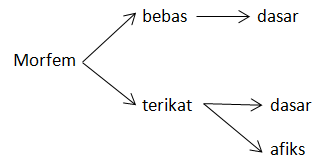
\includegraphics[scale=1]{Gambar/gambar-morfem-bebas-terikat}
	\caption[Morfem bebas dan terikat]{Morfem bebas dan terikat\cite{chaer:08:morfologi}} 
	\label{gambar-morfem-bebas-terikat}
	\end{figure}
	
	Berkenaan dengan bentuk dasar terikat, perlu dikemukakan catatan sebagai berikut:\\
	\textit{Pertama}, bentuk dasar terikat seperti \textit{gaul}, \textit{juang}, dan \textit{henti} lazim juga disebut sebagai \textit{prakategorial} karena bentuk-bentuk tersebut belum memiliki kategori sehingga tidak dapat digunakan dalam pertuturan.\\
	\textit{Kedua}, Verhaar (1978) juga memasukkan bentuk-bentuk seperti \textit{beli}, \textit{baca}, dan \textit{tulis} ke dalam kelompok prakategorial, karena untuk digunakan di dalam kalimat harus terlebih dahulu diberi prefiks \textit{me-}, prefiks \textit{di-}, atau prefiks \textit{ter-}. Dalam kalimat imperatif memang tanpa imbuhan bentuk-bentuk tersebut dapat digunakan. Namun, kalimat imperatif adalah hasil transformasi dari kalimat aktif transitif (yang memerlukan imbuhan).\\
	\textit{Ketiga}, bentuk-bentuk seperti \textit{renta} (yang hanya muncul dalam \textit{tua renta}), \textit{kerontang} (yang hanya muncul dalam \textit{kering kerontang}), dan \textit{kuyup} (yang hanya muncul dalam \textit{basah kuyup}) adalah juga termasuk morfem terikat. Lalu, oleh karena hanya muncul dalam pasangan tertentu, maka disebut \textit{morfem unik}.\\
	\textit{Keempat}, bentuk-bentuk yang disebut klitika merupakan morfem yang agak sukar ditentukan statusnya, apakah morfem bebas atau morfem terikat. Kemunculannya dalam pertuturan selalu terikat dengan bentuk lain, tetapi dapat dipisahkan. Umpamanya klitika \textit{-ku} dalam konstruksi \textit{bukuku} dapat dipisahkan sehingga menjadi \textit{buku baruku}. Dilihat dari posisi tempatnya dibedakan adanya proklitika, yaitu klitika yang berposisi di muka kata yang diikuti seperti klitika \textit{ku-} dalam bentuk \textit{kubawa} dan \textit{kauambil}. Sedangkan yang disebut enklitika adalah klitika yang berposisi di belakang kata yang dilekati, seperti klitika \textit{-mu} dan \textit{-nya} pada bentuk \textit{nasibmu} dan \textit{duduknya}.\\
	\textit{Kelima}, bentuk-bentuk yang termasuk preposisi dan konjungsi seperti \textit{dan}, \textit{oleh}, \textit{di}, dan \textit{karena} secara morfologis termasuk morfem bebas, tetapi secara sintaksis merupakan bentuk terikat (dalam satuan sintaksisnya).\\
	\textit{Keenam}, bentuk-bentuk yang oleh Kridalaksana (1989) disebut proleksem, seperti \textit{a} (pada \textit{asusila}), \textit{dwi} (pada \textit{dwibahasa}), dan \textit{ko} (pada \textit{kopilot}) juga termasuk morfem terikat.
	
	\item Berdasarkan keutuhan bentuknya dibedakan adanya \textit{morfem utuh} dan \textit{morfem terbagi}. Morfem utuh secara fisik merupakan satu-kesatuan yang utuh. Semua morfem dasar, baik bebas maupun terikat, serta prefiks, infiks, dan sufiks termasuk morfem utuh. Sedangkan yang dimaksud morfem terbagi adalah morfem yang fisiknya terbagi atau disisipi morfem lain. Karenanya semua konfiks (seperti \textit{pe-an}, \textit{ke-an}, dan \textit{per-an}) adalah termasuk morfem terbagi. \\
	Namun, mengenai morfem terbagi ini ada dua catatan yang perlu diperhatikan.\\
	\textit{Pertama}, semua konfiks adalah morfem terbagi; tetapi pada bentuk \textit{ber-an} ada yang berupa konfiks dan ada yang bukan konfiks. Jika kata dalam bentuk \textit{ber-an} tidak memiliki arti ketika hanya ditambahkan prefiks \textit{ber-} atau sufiks \textit{-an} saja, maka bentuk \textit{ber-an} tersebut adalah berupa konfiks. Namun, jika kata tersebut memiliki arti ketika hanya ditambahkan prefiks \textit{ber-} atau sufiks \textit{-an} saja, maka bentuk \textit{ber-an} tersebut adalah berupa \textit{klofiks} (akronim dari kelompok afiks). Contoh, kata \textit{bermunculan} adalah dasar \textit{muncul} ditambahkan konfiks \textit{ber-an} sementara kata \textit{berpakaian} adalah prefiks \textit{ber-} yang ditambahkan pada bentuk \textit{pakaian}.\\
	\textit{Kedua}, dalam bahasa Indonesia ada afiks yang disebut infiks, yaitu afiks yang ditempatkan di tengah (di dalam kata). Umpamanya infiks \textit{-el-} pada dasar \textit{tunjuk} menjadi kata \textit{telunjuk}. Di sini infiks itu memecah morfem \textit{tunjuk} menjadi dua bagian, yaitu \textit{t-el-unjuk}. Dengan demikian morfem \textit{t-unjuk} menjadi morfem terbagi, bukan morfem utuh.
	
	\item Berdasarkan kemungkinan menjadi dasar dalam pembentukan kata, dibedakan \textit{morfem dasar} dan \textit{morfem afiks}. Morfem dasar adalah morfem yang dapat menjadi dasar dalam suatu proses morfologi. Misalnya, morfem $\lbrace$beli$\rbrace$, $\lbrace$makan$\rbrace$, dan $\lbrace$merah$\rbrace$. Namun, perlu dicatat bentuk dasar yang termasuk dalam kategori preposisi dan konjungsi tidak pernah mengalami proses afiksasi. Sedangkan, yang tidak dapat menjadi dasar, melainkan hanya sebagai pembentuk disebut morfem afiks, seperti morfem $\lbrace$me-$\rbrace$, $\lbrace$-kan$\rbrace$, dan $\lbrace$pe-an$\rbrace$. Berdasarkan pembagian ini, maka dapat dibuat gambar \ref{gambar-morfem-dasar-afiks} berikut.
	
	\begin{figure}[H]
	\centering
	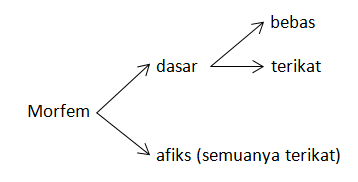
\includegraphics[scale=1]{Gambar/gambar-morfem-dasar-afiks}
	\caption[Morfem dasar dan afiks]{Morfem dasar dan afiks\cite{chaer:08:morfologi}} 
	\label{gambar-morfem-dasar-afiks}
	\end{figure}
	
	%\item Berdasarkan jenis fonem yang membentuknya dibedakan adanya \textit{morfem segmental} dan \textit{morfem suprasegmental} atau \textit{morfem nonsegmental}. Morfem segmental adalah morfem yang dibentuk oleh fonem-fonem segmental, yakni morfem yang berupa bunyi dan dapat disegmentasikan. Misalnya morfem $\lbrace$lihat$\rbrace$, $\lbrace$ter-$\rbrace$, $\lbrace$sikat$\rbrace$, dan $\lbrace$-lah$\rbrace$. Sedangkan morfem suprasegmental adalah morfem yang terbentuk dari nada, tekanan, durasi, dan intonasi. Dalam bahasa Indonesia tidak ditemukan morfem suprasegmental ini; tetapi dalam bahasa Cina, Thai, dan Burma morfem tersebut kita dapati.
	
	\item Berdasarkan ciri semantik dibedakan adanya \textit{morfem bermakna leksikal} dan \textit{morfem tak bermakna leksikal}. Sebuah morfem disebut bermakna leksikal karena di dalam dirinya, secara inheren, telah memiliki makna. Semua morfem dasar bebas, seperti $\lbrace$makan$\rbrace$, $\lbrace$pulang$\rbrace$, dan $\lbrace$pergi$\rbrace$ termasuk morfem bermakna leksikal. Sebaliknya, morfem afiks seperti $\lbrace$ber-$\rbrace$, $\lbrace$ke-$\rbrace$, dan $\lbrace$ter-$\rbrace$ termasuk morfem tak bermakna leksikal. Morfem bermakna leksikal dapat langsung menjadi unsur dalam pertuturan, sementara morfem tidak bermakna leksikal tidak dapat. 
	
\end{enumerate}

Dikotomi morfem bermakna leksikal dan tidak bermakna leksikal ini, untuk bahasa Indonesia timbul masalah. Morfem-morfem seperti $\lbrace$juang$\rbrace$, $\lbrace$henti$\rbrace$, dan $\lbrace$gaul$\rbrace$ memiliki makna leksikal atau tidak. Kalau dikatakan memiliki makna leksikal, pada kenyataannya morfem-morfem itu belum dapat digunakan dalam pertuturan sebelum mengalami proses morfologi. Kalau dikatakan tidak bermakna leksikal, pada kenyataannya morfem-morfem tersebut bukan afiks.

%Dalam hal ini perlu dibedakan antara konsep atau kategori gramatika dengan kategori semantik. Secara gramatikal bentuk-bentuk tersebut memang tidak dapat langsung digunakan dalam sebuah pertuturan. Namun, secara semantik bentuk-bentuk tersebut tetap memiliki makna leksikal.

%Ada satu masalah lagi berkenaan dengan morfem bermakna leksikal ini, yaitu morfem-morfem yang berkategori gramatikal sebagai preposisi dan konjungsi. Banyak pakar (seperti Keraf 1986 dan Parera 1988) yang menyatakan bahwa kelas-kelas preposisi dan konjungsi tidak memiliki makna leksikal, dan hanya mempunyai fungsi gramatikal. Sebenarnya sebagai morfem dasar, dan bukan afiks, semua morfem preposisi dan konjungsi memiliki makna leksikal. Namun, kebebasannya dalam pertuturan memang terbatas. Meskipun keterbatasannya tidak seketat morfem afiks. Dalam morfologi morfem-morfem yang termasuk preposisi dan konjungsi memiliki kebebasan seperti morfem bebas lainnya; hanya secara sintaksis keduanya terikat pada satuan sintaksisnya.


\subsection{Morfem Dasar, Bentuk Dasar, Akar, dan Leksem}
\label{sec:morfemDasarDLL}

Morfem dasar, bentuk dasar (lebih lazim dasar (\textit{base}) saja), akar, dan leksem adalah empat istilah yang lazim digunakan dalam kajian morfologi. Namun, seringkali digunakan secara kurang cermat, malah seringkali berbeda. Oleh karena itu, ada baiknya istilah-istilah tersebut dibicarakan dulu sebelum pembicaraan mengenai proses-proses morfologi.

Istilah \textit{morfem dasar} biasanya digunakan sebagai dikotomi dengan morfem afiks. Jadi, bentuk-bentuk seperti $\lbrace$beli$\rbrace$, $\lbrace$juang$\rbrace$, dan $\lbrace$kucing$\rbrace$ adalah morfem dasar. Morfem dasar ini ada yang termasuk morfem bebas seperti $\lbrace$beli$\rbrace$, $\lbrace$kucing$\rbrace$, dan $\lbrace$pulang$\rbrace$; tetapi ada pula yang termasuk morfem terikat, seperti $\lbrace$juang$\rbrace$, $\lbrace$henti$\rbrace$, dan $\lbrace$tempur$\rbrace$. Sedangkan morfem afiks seperti \textit{$\lbrace$ber-$\rbrace$}, \textit{$\lbrace$di-$\rbrace$}, dan \textit{$\lbrace$-an$\rbrace$} jelas semuanya termasuk morfem terikat seperti dijelaskan pada gambar \ref{gambar-morfem-dasar-afiks} di atas.

Sebuah morfem dasar dapat menjadi bentuk dasar atau dasar (\textit{base}) dalam suatu proses morfologi. Artinya, morfem dasar dapat diberi afiks tertentu dalam proses afiksasi, dapat diulang dalam proses reduplikasi, atau dapat digabung dengan morfem yang lain dalam suatu proses komposisi atau pemajemukan.

Istilah \textit{bentuk dasar} atau \textit{dasar (base)} biasanya digunakan untuk menyebut sebuah bentuk yang menjadi dasar dalam suatu proses morfologi. Bentuk dasar ini dapat berupa morfem tunggal, tetapi dapat juga berupa gabungan morfem. Umpamanya pada kata \textit{berbicara} yang terdiri dari morfem $\lbrace$ber-$\rbrace$ dan morfem $\lbrace$bicara$\rbrace$; maka morfem $\lbrace$bicara$\rbrace$ adalah menjadi bentuk dasar dari kata \textit{berbicara} itu, yang kebetulan juga berupa morfem dasar. Pada kata \textit{dimengerti} bentuk dasarnya adalah \textit{mengerti}, dan pada kata \textit{keanekaragaman} bentuk dasarnya adalah \textit{aneka ragam}. Pada bentuk reduplikasi \textit{rumah-rumah} bentuk dasarnya adalah \textit{rumah}, pada bentuk reduplikasi \textit{berlari-lari} bentuk dasarnya berlari, dan pada bentuk reduplikasi \textit{kemerah-merahan} bentuk dasarnya adalah \textit{kemerahan}. Lalu, pada komposisi \textit{sate ayam} bentuk dasarnya adalah \textit{sate}, pada komposisi \textit{ayam betina} bentuk dasarnya adalah \textit{ayam}, dan pada komposisi \textit{pasar induk} bentuk dasarnya adalah \textit{pasar}. Jadi, bentuk dasar adalah bentuk yang langsung menjadi dasar dalam suatu proses morfologi. Wujudnya dapat berupa morfem tunggal, dapat juga berupa bentuk polimorfemis (terdiri dari dua morfem atau lebih).

%Istilah \textit{pangkal} atau \textit{stem} digunakan untuk menyebut bentuk dasar dalam proses pembentukan kata inflektif, atau pembubuhan afiks inflektif. Hal ini terutama terjadi pada bahasa-bahasa fleksi, seperti bahasa Arab, bahasa Itali, bahasa Jerman, dan bahasa Prancis. Dalam bahasa Indonesia proses pembentukan kata inflektif hanya terjadi pada proses pembentukan verba transitif, yakni verba yang berprefiks \textit{me-} (yang dapat diganti dengan \textit{di-}, prefiks \textit{ter-}, dan prefiks zero). Misalnya, pada kata \textit{membeli} pangkalnya adalah \textit{beli}, pada kata \textit{mendaratkan} pangkalnya adalah \textit{daratkan}, dan pada kata \textit{menangisi} pangkalnya adalah bentuk \textit{tangisi}.

Istilah \textit{akar (root)} digunakan untuk menyebut bentuk yang tidak dapat dianalisis lebih jauh lagi. Artinya, akar adalah bentuk yang tersisa setelah semua afiksnya ditanggalkan. Misalkan pada kata \textit{memberlakukan} setelah semua afiksnya ditanggalkan (yaitu prefiks \textit{me-}, prefiks \textit{ber-}, dan sufiks \textit{-kan}) dengan cara tertentu, maka yang tersisa adalah akar \textit{laku}. Akar \textit{laku} ini tidak dapat dianalisis lebih jauh lagi tanpa merusak makna akar tersebut. Contoh lain, kata \textit{keberterimaan} kalau semua afiksnya ditanggalkan akan tersisa akarnya yaitu bentuk \textit{terima}. Bentuk \textit{terima} ini pun tidak dapat dianalisis lebih jauh lagi.

Istilah \textit{leksem} ada digunakan dalam dua bidang kajian linguistik, yaitu bidang \textit{morfologi} dan bidang \textit{semantik}. Dalam kajian morfologi, leksem digunakan untuk mewadahi konsep "bentuk yang akan menjadi kata" melalui proses morfologi. Umpamanya bentuk PUKUL (dalam konvensi 'morfologi' leksem ditulis dengan huruf kapital semua) adalah sebuah leksem yang akan menurunkan kata-kata seperti \textit{memukul}, \textit{dipukul}, \textit{terpukul}, \textit{pukulan}, \textit{pemukul}, dan \textit{pemukulan}. Sedangkan dalam kajian semantik leksem adalah satuan bahasa yang memiliki sebuah makna. Jadi, bentuk-bentuk seperti \textit{kucing}, \textit{membaca}, \textit{matahari}, \textit{membanting tulang}, dan \textit{sumpah serapah} adalah leksem.

Dari bentuk \textit{leksem} ada bentuk-bentuk turunannya, yaitu \textit{leksikon}, \textit{leksikal}, \textit{leksikologi}, dan \textit{leksikografi}. Istilah leksikon dalam arti 'kumpulan leksem' dapat dipadankan dengan istilah \textit{kosakata} atau \textit{perbendaharaan kata}.


\subsection{Morfem Afiks}
\label{sec:morfemAfiks}

Sudah dijelaskan pada subbab \ref{sec:jenisMorfem} bahwa morfem afiks adalah morfem yang tidak dapat menjadi dasar dalam pembentukan kata, tetapi hanya menjadi unsur pembentuk dalam proses afiksasi. Dalam bahasa Indonesia dibedakan adanya morfem afiks yang disebut:

\begin{enumerate}
	\item \textit{Prefiks}, yaitu afiks yang dibubuhkan di kiri bentuk dasar, yaitu prefiks \textit{ber-}, prefiks \textit{me-}, prefiks \textit{per-}, prefiks \textit{pe-}, prefiks \textit{di-}, prefiks \textit{ter-}, prefiks \textit{se-}, dan prefiks \textit{ke-}.
	
	\item \textit{Infiks}, yaitu afiks yang dibubuhkan di tengah kata, biasanya pada suku awal kata, yaitu infiks \textit{-el-}, infiks \textit{-em-}, dan infiks \textit{-er-}.
	
	\item \textit{Sufiks}, adalah afiks yang dibubuhkan di kanan bentuk dasar, yaitu sufiks \textit{-kan}, sufiks \textit{-i}, dan sufiks \textit{-an}.
	
	\item \textit{Konfiks}, yaitu afiks yang dibubuhkan di kiri dan di kanan bentuk dasar secara bersamaan karena konfiks ini merupakan satu kesatuan afiks. Konfiks yang ada dalam bahasa Indonesia adalah konfiks \textit{ke-an}, konfiks \textit{ber-an}, konfiks \textit{pe-an}, konfiks \textit{per-an}, dan konfiks \textit{se-nya}.
	
	\item \textit{Klitika}\footnote{$id.wikibooks.org/wiki/Bahasa\_Indonesia/Klitika$}, adalah imbuhan yang dalam ucapan tidak mempunyai tekanan sendiri dan tidak merupakan kata karena tidak dapat berdiri sendiri. Jadi, klitika merupakan bentuk yang selalu terikat pada bentuk (kata) lain. Dilihat dari posisi tempatnya, dibedakan adanya \textit{proklitika}, yaitu klitika yang berposisi di sebelah kiri kata yang diikuti seperti klitika \textit{ku-} dan \textit{kau-} dalam bentuk \textit{kubawa} dan \textit{kauambil}. Sedangkan yang disebut \textit{enklitika} adalah klitika yang berposisi di belakang kata yang dilekati, seperti klitika \textit{-ku}, \textit{-mu}, \textit{-nya}, dan \textit{-lah} pada bentuk \textit{bukuku}, \textit{nasibmu}, \textit{duduknya}, dan \textit{pergilah}. Ada juga bentuk klitika yang ditulis terpisah dari kata yang diimbuhkan, yaitu klitika \textit{pun} pada bentuk \textit{kami pun}.
	
	\item Dalam bahasa Indonesia ada bentuk kata yang \textit{berklofiks}, yaitu kata yang dibubuhi afiks pada kiri dan kanannya; tetapi pembubuhannya itu tidak sekaligus, melainkan bertahap. Kata-kata berklofiks dalam bahasa Indonesia adalah yang berbentuk \textit{me-kan}, \textit{me-i}, \textit{memper-}, \textit{memper-kan}, \textit{memper-i}, \textit{ber-kan}, \textit{di-kan}, \textit{di-i}, \textit{diper-}, \textit{diper-kan}, \textit{diper-i}, \textit{ter-kan}, dan \textit{ter-i}.
	
	\item Dalam ragam nonbaku ada afiks nasal yang direalisasikan dengan nasal \textit{m-}, \textit{n-}, \textit{ny-}, \textit{ng-}, dan \textit{nge-}. Kridalaksana (1989) menyebut afiks nasal ini dengan istilah \textit{simulfiks}. Contoh: \textit{nulis}, \textit{nyisir}, \textit{ngambil}, dan \textit{ngecat}.
\end{enumerate}


\section{Proses Morfologi}
\label{sec:prosesMorfologi}

Proses morfologi pada dasarnya adalah proses pembentukan kata dari sebuah bentuk dasar melalui pembubuhan afiks (dalam proses afiksasi), pengulangan (dalam proses reduplikasi), dan penggabungan (dalam proses komposisi)\cite{chaer:08:morfologi}. Prosedur ini berbeda dengan analisis morfologi yang mencerai-ceraikan kata (sebagai satuan sintaksis) menjadi bagian-bagian atau satuan-satuan yang lebih kecil. Sebagai contoh, jika dilakukan analisis morfologi terhadap kata \textit{berpakaian}, mula-mula kata \textit{berpakaian} dianalisis menjadi bentuk \textit{ber-} dan \textit{pakaian}; lalu bentuk \textit{pakaian} dianalisis lagi menjadi bentuk \textit{pakai} dan \textit{-an}. Dalam proses morfologi, prosedurnya dibalik: mula-mula dasar \textit{pakai} diberi sufiks \textit{-an} menjadi \textit{pakaian}. Kemudian kata \textit{pakaian} itu diberi prefiks \textit{ber-} menjadi \textit{berpakaian}. Jadi, kalau analisis morfologi mencerai-ceraikan data kebahasaan yang ada, sedangkan proses morfologi mencoba menyusun dari komponen-komponen kecil menjadi sebuah bentuk yang lebih besar yang berupa kata kompleks atau kata yang polimorfemis.

Proses morfologi melibatkan komponen bentuk dasar dan alat pembentuk kata (afiksasi, reduplikasi, dan komposisi).% (3) makna gramatikal, dan (4) hasil proses pembentukan.


\subsection{Bentuk Dasar}
\label{sec:bentukDasar}

Pada subbab \ref{sec:morfemDasarDLL} telah disinggung bahwa \textit{bentuk dasar} adalah bentuk yang kepadanya dilakukan proses morfologi. Bentuk dasar dapat berupa akar seperti \textit{baca}, \textit{pahat}, dan \textit{juang} pada kata \textit{membaca}, \textit{memahat}, dan \textit{berjuang}. Dapat pula berupa bentuk polimorfemis seperti bentuk \textit{bermakna}, \textit{berlari}, dan \textit{jual beli} pada kata \textit{kebermaknaan}, \textit{berlari-lari}, dan \textit{berjual beli}.

Dalam proses reduplikasi, bentuk dasar dapat berupa akar, seperti akar \textit{rumah} pada kata \textit{rumah-rumah}, akar \textit{tinggi} seperti pada kata \textit{tinggi-tinggi}, dan akar \textit{marah} pada kata \textit{marah-marah}. Dapat juga berupa kata berimbuhan seperti \textit{menembak} pada kata \textit{menembak-nembak}, kata berimbuhan \textit{bangunan} pada kata \textit{bangunan-bangunan}, dan kata berimbuhan \textit{kemerahan} pada kata \textit{kemerah-merahan}. Dapat juga berupa kata gabung seperti \textit{rumah sakit} pada kata \textit{rumah-rumah sakit}, dan \textit{anak nakal} pada kata \textit{anak-anak nakal}.

Dalam proses komposisi, bentuk dasar dapat berupa akar \textit{sate} pada kata \textit{sate ayam}, \textit{sate padang}, dan \textit{sate lontong}; dapat berupa dua buah akar seperti akar \textit{kampung} dan akar \textit{halaman} pada kata \textit{kampung halaman}, atau akar \textit{tua} dan akar \textit{muda} pada kata \textit{tua muda}.

Ada perbedaan bentuk antara \textit{pelajar} dan \textit{pengajar}. Menurut kajian tradisional dan struktural bentuk dasar dari kedua kata itu adalah sama, yaitu akar \textit{ajar}. Dalam kajian proses di sini bentuk dasar kedua kata itu tidaklah sama. Bentuk dasar kata \textit{pelajar} adalah \textit{belajar} sedangkan bentuk dasar kata \textit{pengajar} adalah \textit{mengajar}. Ini dikarenakan makna gramatikal kata \textit{pelajar} adalah 'orang yang belajar' sedangkan makna gramatikal kata \textit{pengajar} adalah 'orang yang mengajar'. Contoh lain, bentuk dasar kata \textit{penyatuan} adalah \textit{menyatukan} karena makna \textit{penyatuan} adalah 'hal/proses menyatukan'. Sedangkan bentuk dasar kata \textit{persatuan} adalah \textit{bersatu} atau \textit{mempersatukan} karena makna gramatikalnya adalah 'hal bersatu' atau 'hal mempersatukan'. Namun, secara teoretis dapat juga dikatakan bentuk dasar kata \textit{pelajar} dan \textit{pengajar} adalah sama yaitu \textit{ajar}; tetapi bentuk \textit{pelajar} dibentuk dari dasar ajar melalui verba \textit{belajar}, sedangkan \textit{pengajar} dibentuk dari dasar \textit{ajar} melalui verba \textit{mengajar}. Demikian juga kata \textit{penyatuan} dibentuk dari dasar \textit{satu} melalui verba \textit{menyatukan}, sedangkan kata \textit{persatuan} dibentuk dari dasar \textit{satu} melalui verba \textit{bersatu} atau \textit{mempersatukan}.

Dari uraian di atas, jelas bahwa konsep \textit{bentuk dasar} tidak sama dengan pengertian \textit{morfem dasar} atau \textit{kata dasar}. Ini dikarenakan bentuk dasar dapat juga berupa bentuk-bentuk polimorfemis.


\subsection{Pembentuk Kata}
\label{sec:pembentukKata}

Komponen kedua dalam proses morfologi adalah alat pembentuk kata. Sejauh ini alat pembentuk kata dalam proses morfologi adalah (a) afiks dalam proses afiksasi, (b) pengulangan dalam proses reduplikasi, dan (c) penggabungan dalam proses komposisi.

Dalam proses afiksasi sebuah afiks diimbuhkan pada bentuk dasar sehingga hasilnya menjadi sebuah kata. Umpamanya pada dasar \textit{baca} diimbuhkan afiks \textit{me-} sehingga menghasilkan kata \textit{membaca} yaitu sebuah verba transitif aktif; pada dasar \textit{juang} diimbuhkan afiks \textit{ber-} sehingga menghasilkan verba intransitif \textit{berjuang}.

Berkenaan dengan jenis afiksnya, proses afiksasi dibedakan atas \textit{prefiksasi}, yaitu proses pembubuhan prefiks, \textit{konfiksasi} yakni proses pembubuhan konfiks, \textit{sufiksasi} yaitu proses pembubuhan sufiks dan \textit{infiksasi} yakni proses pembubuhan infiks. Perlu dicatat dalam bahasa Indonesia proses infiksasi sudah tidak produktif lagi. Dalam hal ini perlu juga diperhatikan adanya \textit{klofiksasi}, yaitu kelompok afiks yang proses afiksasinya dilakukan bertahap. Misalnya pembentukan kata \textit{menangisi}, mula-mula pada dasar \textit{tangis} diimbuhkan sufiks \textit{-i}; setelah itu baru dibubuhkan prefiks \textit{me-}.

Proses prefiksasi dilakukan oleh prefiks \textit{ber-}, \textit{me-}, \textit{pe-}, \textit{per-}, \textit{di-}, \textit{ter-}, \textit{ke-}, dan \textit{se-}; infiksasi dilakukan oleh infiks \textit{-el-}, \textit{-em-}, dan \textit{-er-}; sufiksasi dilakukan sufiks \textit{-an}, \textit{-kan}, dan \textit{-i}; konfiksasi dilakukan oleh konfiks \textit{pe-an}, \textit{per-an}, \textit{ke-an}, \textit{se-nya}, dan \textit{ber-an}; dan klofiksasi dilakukan oleh klofiks \textit{me-kan}, \textit{me-i}, \textit{memper-}, \textit{memper-kan}, \textit{memper-i}, \textit{ber-kan}, \textit{di-kan}, \textit{di-i}, \textit{diper-}, \textit{diper-kan}, \textit{diper-i}, \textit{ter-kan}, dan \textit{ter-i}.

%Namun, perlu dicatat ada afiks yang sangat produktif yaitu prefiks \textit{ber-} dan prefiks \textit{me-}; ada yang cukup produktif, yaitu prefiks \textit{ter-}, sufiks \textit{-kan}, sufiks \textit{-i}, dan sufiks -an; dan juga ada yang tidak produktif lagi, yaitu infiks \textit{-el-}, \textit{-em-}, dan \textit{-er-}.

Alat pembentuk kedua adalah pengulangan bentuk dasar yang digunakan dalam proses reduplikasi. Hasil dari proses reduplikasi ini lazim disebut dengan istilah \textit{kata ulang}. Secara umum dikenal adanya tiga macam pengulangan, yaitu pengulangan secara utuh, pengulangan dengan pengubahan bunyi vokal maupun konsonan, dan pengulangan sebagian.

Alat pembentuk ketiga adalah penggabungan sebuah bentuk pada bentuk dasar yang ada dalam proses komposisi. Penggabungan ini juga merupakan alat yang banyak digunakan dalam pembentukan kata karena banyaknya konsep yang belum ada wadahnya dalam bentuk sebuah kata. Misalnya, bahasa Indonesia hanya punya sebuah kata untuk berbagai macam warna merah. Oleh karena itulah dibentuk gabungan kata seperti \textit{merah jambu}, \textit{merah darah}, dan \textit{merah bata}.

%Alat pembentuk keempat adalah abreviasi khusus yang digunakan dalam proses akronimisasi. Disebut abreviasi khusus karena semua abreviasi menghasilkan akronim. Abreviasi dari bentuk \textit{Sekolah Menengah Atas} menjadi SMA adalah bukan akronim; tetapi hasil abreviasi dari \textit{Jakarta Bogor Ciawi} menjadi \textit{Jagorawi} adalah akronim.

%Alat kelima dalam pembentukan kata adalah pengubahan status dalam proses yang disebut konversi. Misalnya, bentuk \textit{gunting} yang berstatus nomina dalam kalimat "gunting ini terbuat dari baja", dapat diubah statusnya menjadi bentuk \textit{gunting} yang berstatus verba, seperti dalam kalimat "gunting dulu baik-baik, nanti baru dilem".


%\subsection{Hasil Proses Pembentukan}
%\label{sec:hasilProsesPembentukan}

%Proses morfologi atau proses pembentukan kata mempunyai dua hasil yaitu \textit{bentuk} dan \textit{makna gramatikal}. Bentuk dan makna gramatikal merupakan dua hal yang berkaitan erat; bentuk merupakan wujud fisiknya dan makna gramatikal merupakan isi dari wujud fisik atau bentuk itu.

%Wujud fisik dari hasil proses afiksasi adalah kata berafiks, disebut juga kata berimbuhan, kata turunan, atau kata terbitan. Wujud fisik dari proses reduplikasi adalah kata ulang, atau disebut juga bentuk ulang. Wujud fisik dari hasil proses komposisi adalah kata gabung, disebut juga gabungan kata, kelompok kata, atau kata majemuk.% (tentang istilah kata majemuk banyak menimbulkan persoalan. Nanti, akan dibahas tersendiri pada subbab lainnya).


\section{Morfofonemik}
\label{sec:morfofonemik}

Morfofonemik (disebut juga morfofonologi) adalah kajian mengenai terjadinya perubahan bunyi atau perubahan fonem sebagai akibat dari adanya proses morfologi, baik proses afiksasi, proses reduplikasi, maupun proses komposisi\cite{chaer:08:morfologi}. Morfofonemik dalam pembentukan kata bahasa Indonesia terutama terjadi dalam proses afiksasi. Dalam proses reduplikasi dan komposisi hampir tidak ada. Dalam proses afiksasi pun terutama, hanya dalam prefiksasi \textit{ber-}, prefiksasi \textit{me-}, prefiksasi \textit{pe-}, prefiksasi \textit{per-}, konfiksasi \textit{pe-an}, konfiksasi \textit{per-an}, dan sufiksasi \textit{-an}. 

Berikut adalah beberapa jenis perubahan fonem dan bentuk-bentuk morfofonemik pada beberapa proses morfologi.

%Umpamanya, dalam proses pengimbuhan sufiks \textit{-an} pada dasar \textit{hari} akan muncul bunyi [y], yang dalam ortografi tidak dituliskan, tetapi dalam ucapan dituliskan. 

%\begin{center}
%$Hari + an \rightarrow [hariyan]$
%\end{center}

%Contoh lain, dalam proses pengimbuhan sufiks \textit{-an} pada dasar \textit{jawab} akan terjadi pergeseran letak bunyi [b] kebelakang, membentuk suku kata baru.

%\begin{center}
%$Ja.wab + an \rightarrow [ja.wa.ban]$
%\end{center}

%Morfofonemik dalam pembentukan kata bahasa Indonesia terutama terjadi dalam proses afiksasi. Dalam proses reduplikasi dan komposisi hampir tidak ada. Dalam proses afiksasi pun terutama, hanya dalam prefiksasi \textit{ber-}, prefiksasi \textit{me-}, prefiksasi \textit{pe-}, prefiksasi \textit{per-}, prefiksasi \textit{ter-}, konfiksasi \textit{pe-an}, konfiksasi \textit{per-an}.

\subsection{Jenis Perubahan}
\label{sec:jenisPerubahan}

Dalam bahasa Indonesia ada beberapa jenis perubahan fonem berkenaan dengan proses morfologi ini. Di antaranya adalah proses:

\begin{enumerate}

	\item \textit{Pemunculan fonem}, yakni munculnya fonem (bunyi) dalam proses morfologi yang pada mulanya tidak ada. Misalnya, dalam proses pengimbuhan prefiks \textit{me-} pada dasar \textit{baca} akan memunculkan bunyi sengau [m] yang semula tidak ada.\\
	$me + baca \rightarrow membaca$
	
	\item \textit{Pelesapan fonem}, yakni hilangnya fonem dalam suatu proses morfologi. Misalnya, dalam proses pengimbuhan prefiks \textit{ber-} pada dasar \textit{renang}, maka bunyi [r] yang ada pada prefiks \textit{ber-} dilesapkan. Juga, dalam proses pengimbuhan "akhiran" \textit{-wan} pada dasar \textit{sejarah}, maka fonem /h/ pada dasar \textit{sejarah} itu dilesapkan. Contoh lain, pada proses pengimbuhan "akhiran" \textit{-nda} pada dasar \textit{anak}, maka fonem /k/ pada dasar \textit{anak} dilesapkan atau dihilangkan.\\
	$ber + renang \rightarrow berenang$\\
	$sejarah + wan \rightarrow sejarawan$\\
	$anak + nda \rightarrow ananda$
	
	Dalam beberapa tahun terakhir ada juga gejala pelesapan salah satu fonem yang sama yang terdapat pada akhir kata dan awal kata yang mengalami proses komposisi. Misalnya.\\
	$pasar + raya \rightarrow pasaraya$\\
	$ko + operasi \rightarrow koperasi$
	
	\item \textit{Peluluhan fonem}, yakni luluhnya sebuah fonem serta disenyawakan dengan fonem lain dalam suatu proses morfologi. Umpamanya, dalam pengimbuhan prefiks \textit{me-} pada dasar \textit{sikat}, maka fonem /s/ pada kata \textit{sikat} itu diluluhkan dan disenyawakan dengan fonem nasal /ny/ yang ada pada prefiks \textit{me-}. Hal yang sama juga terjadi pada proses pengimbuhan prefiks \textit{pe-}.\\
	$me + sikat \rightarrow menyikat$\\
	$pe + sikat \rightarrow penyikat$
	
	\item \textit{Perubahan fonem}, yakni berubahnya sebuah fonem atau sebuah bunyi, sebagai akibat terjadinya proses morfologi. Umpamanya, dalam pengimbuhan prefiks \textit{ber-} pada dasar \textit{ajar} terjadi perubahan bunyi, di mana fonem /r/ berubah menjadi fonem /l/.\\
	$ber + ajar \rightarrow belajar$

\end{enumerate}


\subsection{Prefiksasi ber-}
\label{sec:prefiksasiBer-}

Morfofonemik dalam proses pengimbuhan prefiks \textit{ber-} berupa: (a) pelesapan fonem /r/ pada prefiks \textit{ber-}; (b) perubahan fonem /r/ pada prefiks \textit{ber-} menjadi fonem /l/; dan (c) pengekalan fonem /r/ yang terdapat prefiks \textit{ber-} itu.

\begin{enumerate}
	\item Pelesapan fonem /r/ pada prefiks \textit{ber-} itu terjadi apabila bentuk dasar yang diimbuhi mulai dengan fonem /r/, atau suku pertama bentuk dasarnya berbunyi [er]. Misalnya:\\
	$ber + renang \rightarrow berenang$\\
	$ber + ragam \rightarrow beragam$\\
	$ber + racun \rightarrow beracun$\\
	$ber + kerja \rightarrow bekerja$\\
	$ber + ternak \rightarrow beternak$\\
	$ber + cermin \rightarrow becermin$
	
	\item Perubahan fonem /r/ pada prefiks \textit{ber-} menjadi fonem /l/ terjadi bila bentuk dasarnya akar \textit{ajar}; tidak ada contoh lain.\\
	$ber + ajar \rightarrow belajar$
	
	\item Pengekalan fonem /r/ pada prefiks \textit{ber-} tetap /r/ terjadi apabila bentuk dasarnya bukan yang ada pada poin 1 dan 2 di atas.\\
	$ber + obat \rightarrow berobat$\\
	$ber + korban \rightarrow berkorban$\\
	$ber + getah \rightarrow bergetah$\\
	$ber + lari \rightarrow berlari$\\
	$ber + tamu \rightarrow bertamu$
	
\end{enumerate}


\subsection{Prefiksasi me- (termasuk klofiks me-kan dan me-i)}
\label{sec:prefiksasiMe-}

Morfofonemik dalam proses pengimbuhan dengan prefiks \textit{me-} dapat berupa: (a) pengekalan fonem; (b) penambahan fonem; dan (c) peluluhan fonem.

\begin{enumerate}
	\item Pengekalan fonem di sini artinya tidak ada fonem yang berubah, tidak ada yang dilesapkan dan tidak ada yang ditambahkan. Hal ini terjadi apabila bentuk dasarnya diawali dengan konsonan /r, l, w, y, m, n, ng, dan ny/. Contoh:\\
	$me + rawat \rightarrow merawat$\\
	$me + lirik \rightarrow melirik$\\
	$me + wasiat \rightarrow wasiat$\\
	$me + yakin \rightarrow meyakinkan$\\
	$me + makan \rightarrow memakan$\\
	$me + nanti \rightarrow menanti$\\
	$me + nganga \rightarrow nganga$\\
	$me + nyanyi \rightarrow nyanyi$
	
	\item Penambahan fonem, yakni penambahan fonem nasal /m, n, ng, dan nge/. Penambahan fonem nasal /m/ terjadi apabila bentuk dasarnya dimulai dengan konsonan /b/, /f/, dan /v/. Umpamanya:\\
	$me + baca \rightarrow membaca$\\
	$me + buru \rightarrow memburu$\\
	$me + fitnah \rightarrow memfitnah$\\
	$me + fokus \rightarrow memfokus (kan)$\\
	$me + vonis \rightarrow memvonis$
	
	Penambahan fonem nasal /n/ terjadi apabila bentuk dasarnya dimulai dengan konsonan /c/, /d/, dan /j/. Umpamanya:\\
	$me + cari \rightarrow mencari$\\
	$me + dengar \rightarrow mendengar$\\
	$me + jual \rightarrow menjual$
	
	Penambahan fonem nasal /ng/ terjadi apabila bentuk dasarnya dimulai dengan konsonan /g, h, dan kh/ dan huruf vokal /a, i, u, e, dan o/. Contoh:\\
	$me + goda \rightarrow menggoda$\\
	$me + hina \rightarrow menghina$\\
	$me + khayal \rightarrow mengkhayal$\\
	$me + ambil \rightarrow mengambil$\\
	$me + iris \rightarrow mengiris$\\
	$me + ukur \rightarrow mengukur$\\
	$me + elak \rightarrow mengelak$\\
	$me + obral \rightarrow mengobral$
	
	Penambahan fonem nasal /nge/ terjadi apabila bentuk dasarnya hanya terdiri dari satu suku kata. Misalnya:\\
	$me + bom \rightarrow mengebom$\\
	$me + cat \rightarrow mengecat$\\
	$me + lap \rightarrow mengelap$
	
	\item Peluluhan fonem terjadi apabila prefiks \textit{me-} diimbuhkan pada bentuk dasar yang dimulai dengan konsonan bersuara /s, k, p, dan t/. Dalam hal ini konsonan /s/ diluluhkan dengan nasal /ny/, konsonan /k/ diluluhkan dengan nasal /ng/, konsonan /p/ diluluhkan dengan nasal /m/, dan konsonan /t/ diluluhkan dengan nasal /n/. Contoh:\\
	$me + sikat \rightarrow menyikat$\\
	$me + kirim \rightarrow mengirim$\\
	$me + pilih \rightarrow memilih$\\
	$me + tolong \rightarrow menolong$
	
\end{enumerate}


\subsection{Prefiksasi pe- dan konfiksasi pe-an}
\label{sec:prefiksasiPe-}

Morfofonemik dalam proses pengimbuhan dengan prefiks \textit{pe-} dan konfiks \textit{pe-an} sama dengan morfofonemik yang terjadi dalam proses pengimbuhan dengan prefiks \textit{me-}, yaitu (a) pengekalan fonem; (b) penambahan fonem; dan (c) peluluhan fonem.

\begin{enumerate}
	\item Pengekalan fonem, artinya tidak ada perubahan fonem, dapat terjadi apabila bentuk dasarnya diawali dengan konsonan /r, l, y, w, m, n, ng, dan ny/. Contoh:\\
	$pe + rawat \rightarrow perawat$\\	
	$pe + latih \rightarrow pelatih$\\
	$pe + yakin \rightarrow peyakin$\\
	$pe + waris \rightarrow pewaris$\\
	$pe-an + manfaat \rightarrow pemanfaatan$\\
	$pe-an + nanti \rightarrow penantian$\\
	$pe + nganga \rightarrow penganga$\\
	$pe + nyanyi \rightarrow penyanyi$
	
	\item Penambahan fonem, yakni penambahan fonem nasal /m, n, ng, dan nge/ antara prefiks dan bentuk dasar. Penambahan fonem nasal /m/ terjadi apabila bentuk dasarnya diawali oleh konsonan /b/. Contoh:\\
	$pe + baca \rightarrow pembaca$\\
	$pe + bina \rightarrow pembina$\\
	$pe + buru \rightarrow pemburu$
	
	Penambahan fonem nasal /n/ terjadi apabila bentuk dasarnya diawali oleh konsonan /c/, /d/, dan /j/. Contoh:\\
	$pe + cari \rightarrow pencari$\\
	$pe + dengar \rightarrow pendengar$\\
	$pe + jual \rightarrow penjual$
	
	Penambahan fonem nasal /ng/ terjadi apabila bentuk dasarnya diawali dengan konsonan /g, h, dan kh/ dan vokal /a, i, u, e, o/. Contoh:\\
	$pe + gali \rightarrow penggali$\\
	$pe + hambat \rightarrow penghambat$\\
	$pe + khianat \rightarrow pengkhianat$\\
	$pe + angkat \rightarrow pengangkat$\\
	$pe + inap \rightarrow penginap$\\
	$pe + usir \rightarrow pengusir$\\
	$pe + elak \rightarrow pengelak$\\
	$pe + obral \rightarrow pengobral$
	
	Penambahan fonem nasal /nge/ terjadi apabila bentuk dasarnya berupa bentuk dasar satu suku. Contoh:\\
	$pe + bom \rightarrow pengebom$\\
	$pe + cat \rightarrow pengecat$\\
	$pe + lap \rightarrow pengelap$
	
	\item Peluluhan fonem, apabila prefiks \textit{pe-} (atau \textit{pe-an}) diimbuhkan pada bentuk dasar yang diawali dengan konsonan tak bersuara /s, k, p, dan t/. Dalam hal ini konsonan /s/ diluluhkan dengan nasal /ny/, konsonan /k/ diluluhkan dengan nasal /ng/, konsonan /p/ diluluhkan dengan nasal /m/, dan konsonan /t/ diluluhkan dengan nasal /n/. Contoh:\\
	$pe + saring \rightarrow penyaring$\\
	$pe + kumpul \rightarrow pengumpul$\\
	$pe + pilih \rightarrow pemilih$\\
	$pe + tulis \rightarrow penulis$
	
\end{enumerate}


\subsection{Prefiksasi per- dan konfiksasi per-an}
\label{sec:prefiksasiPer-}

Morfofonemik dalam pengimbuhan prefiks \textit{per-} dan konfiks \textit{per-an} dapat berupa: (a) pelesapan fonem /r/ pada prefiks \textit{per-} itu; (b) perubahan fonem /r/ dari prefiks \textit{per-} itu menjadi fonem /l/; dan (c) pengekalan fonem /r/ tetap /r/.

\begin{enumerate}
	\item Pelesapan fonem /r/ terjadi apabila bentuk dasarnya dimulai dengan fonem /r/, atau suku kata pertamanya /er/. Contoh:\\
	$per + ringan \rightarrow peringan$\\
	$per + rendah \rightarrow perendah$\\
	$per + ternak \rightarrow peternak$\\
	$per + kerja \rightarrow pekerja$
	
	\item Perubahan fonem /r/ menjadi /l/ terjadi apabila bentuk dasarnya berupa kata \textit{ajar}.\\
	$per + ajar \rightarrow pelajar$
	
	\item Pengekalan fonem /r/ terjadi apabila bentuk dasarnya bukan yang disebutkan pada poin 1 dan 2 di atas. Contoh:\\
	$per + kaya \rightarrow perkaya$\\
	$per + kecil \rightarrow perkecil$\\
	$per + lambat \rightarrow perlambat$\\
	$per + tegas \rightarrow pertegas$	
	
\end{enumerate}


\subsection{Prefiksasi ter-}
\label{sec:prefiksasiTer-}

Morfofonemik dalam proses pengimbuhan dengan prefiks \textit{ter-} dapat berupa: (a) pelesapan fonem /r/ dari prefiks \textit{ter-} itu; (b) perubahan fonem /r/ dari prefiks \textit{ter-} itu menjadi fonem /l/; dan (c) pengekalan fonem /r/ itu. 

\begin{enumerate}
	\item Pelesapan fonem dapat terjadi apabila prefiks \textit{ter-} diimbuhkan pada bentuk dasar yang dimulai dengan konsonan /r/. Misalnya:\\
	$ter + rasa \rightarrow terasa$\\
	$ter + rangkum \rightarrow terangkum$\\
	$ter + rebut \rightarrow terebut$
	
	\item Perubahan fonem /r/ pada prefiks \textit{ter-} menjadi fonem /l/ terjadi apabila prefiks \textit{ter-} itu diimbuhkan pada bentuk dasar \textit{anjur}.\\
	$ter + anjur \rightarrow telanjur$
	
	\item Pengekalan fonem /r/ pada prefiks \textit{ter-} tetap menjadi /r/ apabila prefiks ter- itu diimbuhkan pada bentuk dasar yang bukan disebutkan pada poin 1 dan 2 di atas. Contoh:\\
	$ter + dengar \rightarrow terdengar$\\	
	$ter + jauh \rightarrow terjauh$\\
	$ter + lempar \rightarrow terlempar$\\
	$ter + baik \rightarrow terbaik$
	
\end{enumerate}


\section{Peran Morphological Parser dalam Natural Language Processing\cite{jurafsky:09:nlp}}
\label{sec:peranParser}

Dalam bahasa Inggris, ketika kita ingin menulis sebuah kata benda plural, untuk sebagian besar kasus kita hanya tinggal menambahkan huruf 's' di belakang kata benda yang dimaksud. Misalnya, kita ingin membuat bentuk plural dari kata 'book' kita hanya perlu menambahkan huruf 's' di belakangnya sehingga menjadi kata 'books' yang merupakan bentuk plural dari 'book'. Namun, hal itu tidak berlaku jika kita ingin membuat bentuk plural dari kata 'baby', 'goose', atau 'fish'. Bentuk plural dari kata 'baby', 'goose', dan 'fish' adalah 'babies', 'geese', dan 'fish'. 

%Dibutuhkan dua buah aturan untuk menentukan bentuk singular dan plural dari kata benda tersebut. \textit{Ortographic rules} yang mengatur bahwa kata yang berakhiran huruf 'y' untuk membuat bentuk pluralnya adalah dengan mengganti 'y' dengan 'i' dan menambahkan 'es'. \textit{Morphological rules} yang mengatur bahwa kata 'fish' tidak mempunyai bentuk plural khusus dan kata 'goose' mempunyai bentuk plural dengan mengganti huruf vokalnya. 

Untuk mengenali bentuk 'books' dapat dipisahkan menjadi dua buah morfem 'book' dan 's' diperlukan proses yang disebut dengan \textbf{morphological parsing}. Dalam ranah ilmu temu kembali informasi (\textit{information retrieval}), proses yang sama untuk memetakan bentuk 'books' menjadi 'book' disebut dengan \textit{stemming}. Morphological parsing atau stemming tidak hanya dapat memisahkan bentuk plural dari kata benda, tapi juga dapat untuk bentuk lain seperti bentuk kata kerja berakhiran 'ing' dalam contoh kata 'going', 'talking', dan 'eating'. Ketika dilakukan proses parsing terhadap bentuk tersebut akan didapatkan kata kerja 'go', 'talk', dan 'eat' yang ditambahkan morfem 'ing'. 

Muncul pertanyaan, kenapa kita tidak simpan saja semua bentuk plural dari semua kata benda dan semua bentuk 'ing' dari semua kata kerja dalam bahasa Inggris yang ada dalam kamus? Alasan utamanya adalah karena bentuk 'ing' adalah sufiks yang sangat produktif, yang berarti bentuk tersebut dapat diterapkan pada semua kata kerja. Sama halnya dengan bentuk plural 's' yang bisa diterapkan di hampir semua kata benda. Oleh karena itu, ide untuk menyimpan semua bentuk plural dan bentuk 'ing' akan sangat tidak efisien. 

Morphological parsing dibutuhkan tidak hanya untuk temu kembali informasi. Kita membutuhkan proses tersebut untuk supaya mesin dapat mengerti bahwa kata 'va' dan 'aller' dalam bahasa Perancis keduanya diterjemahkan menjadi kata kerja 'go' dalam bahasa Inggris. Kita juga membutuhkan proses tersebut untuk mengecek ejaan, karena dengan aturan morfologi kita dapat menentukan bahwa kata 'misclam' dan 'antiundoggingly' bukan merupakan kata yang valid dalam bahasa Inggris.


%\section{Finite-State Automata}
%\label{sec:automata}
%
%Automata adalah ...


\section{Struktur Data Trie}
\label{sec:trie}

\textit{Trie} adalah struktur data berupa pohon terurut untuk menyimpan suatu himpunan string di mana setiap node pada pohon tersebut mengandung awalan (prefix) yang sama\cite{najogie:10:trie}. Kata "trie" berasal dari kata \textit{retrieval} yang berarti pengambilan. Struktur data trie ditemukan oleh seorang professor di MIT bernama Edward Fredkin. Trie sering digunakan pada masalah komputasi yang melibatkan penyimpanan dan pencarian string. Trie memiliki sejumlah keunggulan dibanding struktur data lain untuk memecahkan masalah serupa terutama dalam hal kecepatan dan memori yang digunakan.

Dalam trie, tidak ada node yang menyimpan kunci yang terkait dengan node tersebut, sebaliknya, posisinya di pohon menunjukkan kunci apa yang terkait dengannya. Setiap keturunan dari sebuah node memiliki prefix yang sama dengan string yang diwakilkan oleh node tersebut, dan akar menandakan sebuah string kosong.

\begin{figure}[H]
\centering
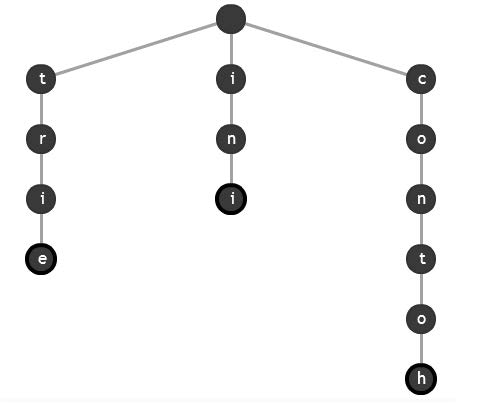
\includegraphics[scale=1]{Gambar/contoh-trie-1}
\caption[Trie]{Trie dengan kata "trie","ini", dan "contoh"\cite{najogie:10:trie}} 
\label{contoh-trie-1}
\end{figure}

Gambar \ref{contoh-trie-1} di atas adalah contoh representasi struktur data trie yang menyimpan tiga buah string, yaitu "trie","ini", dan "contoh". Dari gambar tersebut kita bisa mendapat gambaran mengenai kompleksitas waktu yang diperlukan untuk mencari sebuah kata dalam trie. Jika panjang kata terpanjang dalam trie adalah \textit{L}, maka untuk mencari sebuah kata dalam trie memerlukan waktu terburuk O(\textit{L})

\subsection{Bitwise Trie}
\label{sec:bitwiseTrie}

Bitwise trie adalah salah satu variasi dari trie yang memiliki banyak kesamaan dengan trie berbasis karakter biasa, kecuali dalam representasi dengan bit individual yang biasanya digunakan untuk traversal secara efektif dan membentuk sebuah pohon biner. Secara umum, implementasinya menggunakan fungsi khusus CPU untuk dapat secara cepat mencari himpunan bit dengan panjang tertentu. Nilai ini lalu akan digunakan sebagai entri dari tabel dengan indeks 32 atau 64 yang menunujuk kepada elemen pertama dalam bitwise trie dengan sejumlah bilangan 0 di depan. Proses pencarian selanjutnya akan dilakukan dengan mengetes setiap bit dalam kunci dan memilih anak[0] atau anak[1] sesuai aturan hingga pencarian berakhir.

Walaupun proses ini mungkin terdengar lambat, tetapi sangat fleksibel karena kurangnya ketergantungan terhadap \textit{register} dan oleh karena itu pada kenyataannya melakukan eksekusi dengan sangat baik pada CPU modern.

\subsection{Patricia Trie}
\label{sec:patriciaTrie}

PATRICIA adalah variasi lain dari trie yang merupakan singkatan dari Practical Algorithm To Retrieve Information Coded In Alphanumeric. PATRICIA trie sendiri lebih dikenal dengan sebutan \textit{pohon radix} atau \textit{radix tree}. Pohon radix bisa diartikan secara sederhana sebagai trie yang kompleksitas ruangnya lebih efisien, di mana setiap node yang hanya memiliki satu anak digabung dengan anaknya sendiri. Hasilnya adalah setiap node paling dalam paling tidak memiliki 2 anak. Tidak seperti trie biasa, anak bisa diberi label deretan karakter maupun satu karakter. Ini membuat pohon radix jauh lebih efisien untuk jumlah string yang sedikit (terutama jika stringnya cukup panjang) dan untuk himpunan string yang memiliki prefix sama yang panjang.

\begin{figure}[H]
\centering
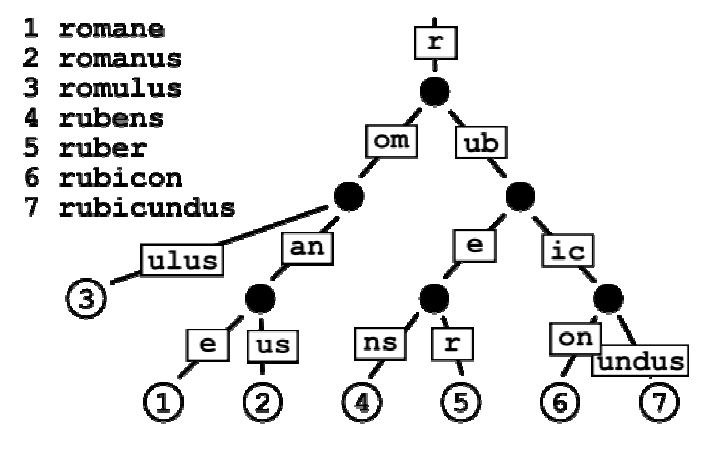
\includegraphics[scale=0.75]{Gambar/contoh-radix-tree}
\caption[Trie]{Pohon radix dengan 7 kata dengan prefix "r"\cite{najogie:10:trie}} 
\label{contoh-radix-tree}
\end{figure}

Pohon radix memiliki fasilitas untuk melakukan operasi-operasi berikut, yang mana setiap operasinya memiliki kompleksitas waktu terburuk O(k), di mana k adalah panjang maksimum string dalam himpunan.

\begin{itemize}
	\item Pencarian: Mencari keberadaan suatu string pada himpunan string. Operasi ini sama dengan pencarian pada trie biasa kecuali beberapa sisi mengandung lebih dari satu karakter.
	\item Penyisipan: Menambahkan sebuah string ke pohon. Kita mencari tempat yang tepat di pohon untuk menyisipkan elemen baru. Jika sudah ada sisi yang memiliki prefix sama dengan string masukan, kita akan memisahkan nya menjadi dua sisi dan memprosesnya. Proses pemisahan ini meyakinkan bahwa tidak ada node yang memiliki anak lebih banyak dari jumlah karakter string yang ada.
	\item Hapus: Menghapus sebuah string dari pohon. Pertama kita menghapus daun yang berkaitan. Lalu, jika orangtuanya hanya memiliki satu anak lagi, kita menghapus orangtuanya dan menggabungkan sisi yang saling terhubung
	\item Cari anak: Mencari string terbesar yang lebih kecil dari string masukan, sesuai dengan urutan alfabet.
	\item Cari orang tua: Mencari string terkecil yang lebih besar dari string masukan, sesuai dengan urutan alfabet.
\end{itemize}

Pengembangan yang umum dari pohon radix yaitu menggunakan node dua warna, hitam dan putih. Untuk mengecek apakah sebuah string masukan sudah ada di dalam pohon, pencarian dimulai dari puncak, dan terus menelusuri setiap sisi sampai tidak ada lagi jalan. Jika node akhir dari proses ini berwarna hitam, berarti pencarian gagal, jika node berwarna putih berarti pencarian telah berhasil. Hal ini membuat kita bisa menambahkan string dalam jumlah banyak yang memiliki prefix yang sama dengan elemen di pohon dengan menggunakan node putih, lalu menghapus sejumlah pengecualian untuk mengehemat memori dengan cara menambahkan elemen string baru dengan node hitam.

\subsection{Implementasi Trie dalam Kamus}
\label{sec:kamus}

Salah satu implementasi dari struktur data trie yang paling populer adalah dalam kamus. Kamus terdiri dari kumpulan kata-kata yang sudah terurut menaik berdasarkan urutan alfabet. Dalam perkembangannya saat ini sudah banyak kamus yang hadir dalam bentuk perangkat lunak, yang bisa digunakan di komputer ataupun di telepon genggam. Kamus dalam bentuk perangkat lunak tentunya memiliki fitur-fitur yang memudahkan pengaksesannya, antara lain pencarian kata dan penambahan kata ke kamus.

Berikut adalah ilustrasi kamus dengan struktur data trie.

\begin{figure}[H]
\centering
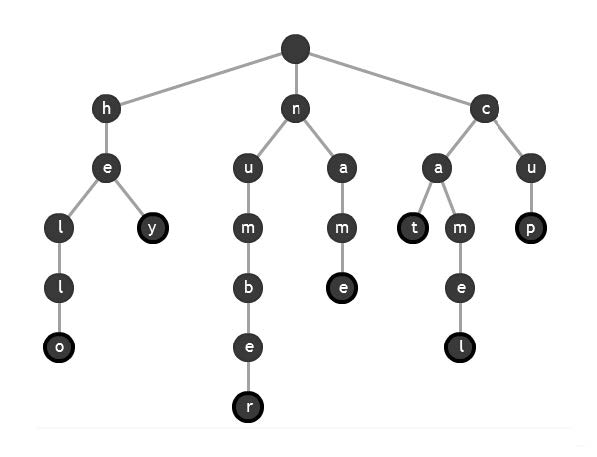
\includegraphics[scale=1.25]{Gambar/contoh-trie-2}
\caption[Trie]{Trie dengan kata "hello","hey","number","name","cat","camel", dan "cup"\cite{najogie:10:trie}} 
\label{contoh-trie-2}
\end{figure}

Dapat dibayangkan, ketika kita mencari sebuah kata dalam kamus, kita akan mulai dengan karakter pertama dari kata tersebut. Jika tidak ada anak dari akar yang nilainya sama dengan karakter itu, maka langsung disimpulkan kata tidak ada di kamus. Jika ada, akan ditelusuri terus sampai ke dasar dari trie, jika kata ditemukan, maka akan dikembalikan info dari node itu, sedangkan jika tidak ketemu kita bisa mengembalikan kata yang memiliki prefix sama dengan kata yang dicari sebagai saran pencarian.

Sementara itu penambahan kata akan berakibat penambahan cabang baru bila kata itu belum ada sebelumnya.

\begin{figure}[H]
\centering
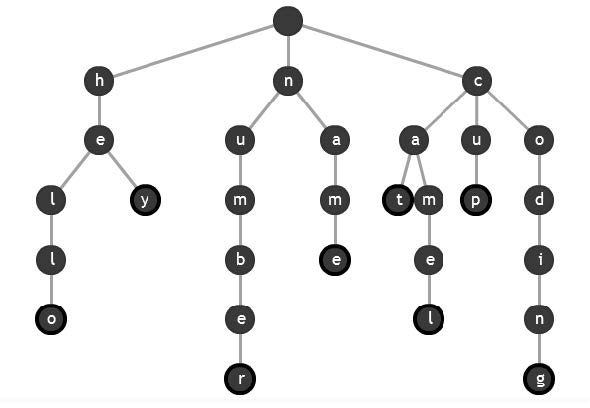
\includegraphics[scale=1.25]{Gambar/contoh-trie-3}
\caption[Trie]{Penambahan kata "coding" pada trie di gambar \ref{contoh-trie-2}\cite{najogie:10:trie}} 
\label{contoh-trie-3}
\end{figure}

\subsection{Keunggulan Trie dibandingkan Struktur Data Lain}
\label{sec:keunggulanTrie}

Trie sebagai turunan dari pohon memiliki keunggulan dibandingkan stuktur data yang sering digunakan untuk persoalan yang sama, yakni pohon pencarian biner dan tabel hash.

Berikut keunggulan utama trie dibandingkan pohon pencarian biner:

\begin{itemize}
	\item Pencarian kunci dengan trie lebih cepat. Mencari sebuah kunci dengan panjang \textit{m} menghabiskan waktu dengan kasus terburuk O(\textit{m}). Pohon pencarian biner melakukan O(log(\textit{n})) perbandingan kunci, dimana \textit{n} adalah jumlah elemen di dalam pohon, karena pencarian pada pohon biner bergantung pada kedalaman pohon, yang mana bernilai logaritmik terhadap jumlah kunci pencarian apabila pohonnya seimbang. Oleh karena itu pada kasus terburuk, sebuah pohon biner menghabiskan waktu O(\textit{m} log \textit{n}), yang mana pada kasus terburuk juga log \textit{n} akan mendekati \textit{m}. Operasi sederhana yang digunakan trie pada saat pencarian karakter, seperti penggunaan array index menggunakan karakter, juga membuat pencarian dengan trie menjadi lebih cepat.
	\item Trie menggunakan ruang lebih sedikit jika memuat string pendek dalam jumlah besar, karena kunci tidak disimpan secara eksplisit dan node dipakai bersama oleh kunci yang memiliki prefix yang serupa.
	\item Trie bisa memiliki fitur untuk menghitung kesamaan prefix terpanjang, yang membantu untuk mencari pengunaan kunci bersama terpanjang dari karakter-karakter yang unik.
\end{itemize}

Berikut keunggulan utama trie dibanding tabel hash:

\begin{itemize}
	\item Trie bisa melakukan pencarian kunci yang paling mirip hampir sama cepatnya dengan pencarian kunci yang tepat, sementara tabel hash hanya bisa mencari kunci yang sama tepat karena tidak menyimpan hubungan antara kunci.
	\item Trie lebih cepat secara rata-rata untuk menyisipkan elemen baru dibandingkan dengan tabel hash. Hal ini terjadi karena tabel hash harus membangun ulang indeksnya ketika tabel sudah penuh, yang mana menghabiskan waktu sangat banyak. Oleh karena itu, trie memiliki kompleksitas waktu terburuk yang batasnya lebih konsisten, yang mana merupakan salah satu unsur penting pada jalannya sebuah program.
	\item Trie bisa diimplementasikan sedemikian sehingga tidak memerlukan memori tambahan. Tabel hash harus selalu memliki memori tambahan untuk menyimpan pengindeksan tabel hash.
	\item Pencarian kunci bisa jauh lebih cepat jika fungsi hashing dapat dihindarkan. Trie bisa menyimpan kunci bertipe integer maupun pointer tanpa perlu membuat fungsi hashing sebelumnya. Hal ini membuat trie lebih cepat daripada tabel hash pada hampir setiap kasus karena fungsi hash yang baik sekalipun cenderung overhead ketika melakukan hashing pada data yang hanya berukuran 4 sampai 8 byte.
	\item Trie bisa menghitung kesamaan prefix terpanjang, sedangkan tabel hash tidak.
\end{itemize}